\documentclass{standalone}
\usepackage{pgfplots}% loads also tikz
\usepackage{physics}

\usetikzlibrary{arrows.meta}
\pgfplotsset{compat=newest} 


\begin{document}

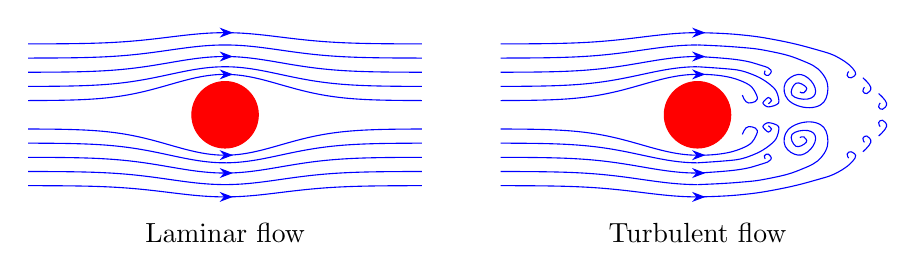
\begin{tikzpicture}
  % balls
  \filldraw[red] (0,0) circle (12pt);
  \filldraw[red] (6,0) circle (12pt);

  % laminar lines
  \def\n{5}
  \foreach \i in{1,...,\n}{
      \draw[thin,blue]  plot [samples=100,domain=-2.5:2.5] ({\x},{1/(\i+2)*exp(-\x*\x)+0.18*\i});
      \draw[thin,blue]  plot [samples=100,domain=-2.5:2.5] ({\x},{-1/(\i+2)*exp(-\x*\x)-0.18*\i});
    }

  % turbulent lines
  \foreach \i in{1,...,\n}{
      \draw[thin,blue]  plot [samples=100,domain=3.5:6] ({\x},{1/(\i+2)*exp(-(\x-6)*(\x-6))+0.18*\i});
      \draw[thin,blue]  plot [samples=100,domain=3.5:6] ({\x},{-1/(\i+2)*exp(-(\x-6)*(\x-6))-0.18*\i});
    }
  %%% upper lines
  \draw [thin, blue] plot [smooth, tension=1] coordinates {(6,0.513) (6.5,0.45) (6.75,0.25) (6.65, 0.15) (6.57,0.25)};
  \draw [thin, blue] plot [smooth, tension=0.5] coordinates {(6,0.61) (6.5,0.57) (6.75,0.49) (6.9, 0.4) (7,0.3) (7.03,0.15) (6.9,0.1) (6.83,0.15) (6.9,0.22) (6.94,0.18) (6.9,0.14)};
  \draw [thin, blue] plot [smooth, tension=0.75] coordinates {(6,0.74) (6.5,0.7) (6.8,0.63) (6.93, 0.57) (6.9,0.5) (6.85,0.52) (6.86,0.56)};
  \draw [thin, blue] plot [smooth, tension=0.75] coordinates {(6,0.887) (6.5,0.86) (6.9,0.81) (7.3, 0.7) (7.58,0.53) (7.65,0.27) (7.5,0.1) (7.2,0.15) (7.1,0.35) (7.23,0.5) (7.4,0.47) (7.5,0.3) (7.4,0.2) (7.2,0.25) (7.25,0.4) (7.38,0.35) (7.35,0.28) (7.3,0.29)};
  \draw [thin, blue] plot [smooth, tension=0.75] coordinates {(6,1.043) (6.5,1.02) (7,0.95) (7.5, 0.83) (7.8,0.72) (8,0.55) (7.95,0.47) (7.9,0.5) (7.92,0.55)};
  \draw [thin, blue] plot [smooth, tension=0.75] coordinates {(7.9 + 0.2,0.67 - 0.2) (8 + 0.2,0.55 - 0.2) (7.95 + 0.2,0.47 - 0.2) (7.9 + 0.2,0.5 - 0.2) (7.92 + 0.2,0.55 - 0.2)};
  \draw [thin, blue] plot [smooth, tension=0.75] coordinates {(7.9 + 0.4,0.67 - 0.4) (8 + 0.4,0.55 - 0.4) (7.95 + 0.4,0.47 - 0.4) (7.9 + 0.4,0.5 - 0.4) (7.92 + 0.4,0.55 - 0.4)};
  %%% lower lines
  \draw [thin, blue] plot [smooth, tension=1] coordinates {(6,-0.513) (6.5,-0.45) (6.75,-0.25) (6.65, -0.15) (6.57,-0.25)};
  \draw [thin, blue] plot [smooth, tension=0.5] coordinates {(6,-0.61) (6.5,-0.57) (6.75,-0.49) (6.9, -0.4) (7,-0.3) (7.03,-0.15) (6.9,-0.1) (6.83,-0.15) (6.9,-0.22) (6.94,-0.18) (6.9,-0.14)};
  \draw [thin, blue] plot [smooth, tension=0.75] coordinates {(6,-0.74) (6.5,-0.7) (6.8,-0.63) (6.93, -0.57) (6.9,-0.5) (6.85,-0.52) (6.86,-0.56)};
  \draw [thin, blue] plot [smooth, tension=0.75] coordinates {(6,-0.887) (6.5,-0.86) (6.9,-0.81) (7.3, -0.7) (7.58,-0.53) (7.65,-0.27) (7.5,-0.1) (7.2,-0.15) (7.1,-0.35) (7.23,-0.5) (7.4,-0.47) (7.5,-0.3) (7.4,-0.2) (7.2,-0.25) (7.25,-0.4) (7.38,-0.35) (7.35,-0.28) (7.3,-0.29)};
  \draw [thin, blue] plot [smooth, tension=0.75] coordinates {(6,-1.043) (6.5,-1.02) (7,-0.95) (7.5, -0.83) (7.8,-0.72) (8,-0.55) (7.95,-0.47) (7.9,-0.5) (7.92,-0.55)};
  \draw [thin, blue] plot [smooth, tension=0.75] coordinates {(7.9 + 0.2,-0.67 + 0.2) (8 + 0.2,-0.55 + 0.2) (7.95 + 0.2,-0.47 + 0.2) (7.9 + 0.2,-0.5 + 0.2) (7.92 + 0.2,-0.55 + 0.2)};
  \draw [thin, blue] plot [smooth, tension=0.75] coordinates {(7.9 + 0.4,-0.67 + 0.4) (8 + 0.4,-0.55 + 0.4) (7.95 + 0.4,-0.47 + 0.4) (7.9 + 0.4,-0.5 + 0.4) (7.92 + 0.4,-0.55 + 0.4)};

  % arrows - laminar 
  \draw[thin,blue,-Stealth] (0,0.513) -- (0.1,0.513);
  \draw[thin,blue,-Stealth] (0,0.74) -- (0.1,0.74);
  \draw[thin,blue,-Stealth] (0,1.043) -- (0.1,1.043);
  \draw[thin,blue,-Stealth] (0,-0.513) -- (0.1,-0.513);
  \draw[thin,blue,-Stealth] (0,-0.74) -- (0.1,-0.74);
  \draw[thin,blue,-Stealth] (0,-1.043) -- (0.1,-1.043);

  % arrows - turbulent 
  \draw[thin,blue,-Stealth] (6,0.513) -- (6.1,0.513);
  \draw[thin,blue,-Stealth] (6,0.74) -- (6.1,0.74);
  \draw[thin,blue,-Stealth] (6,1.043) -- (6.1,1.043);
  \draw[thin,blue,-Stealth] (6,-0.513) -- (6.1,-0.513);
  \draw[thin,blue,-Stealth] (6,-0.74) -- (6.1,-0.74);
  \draw[thin,blue,-Stealth] (6,-1.043) -- (6.1,-1.043);

  % text
  \node at (0,-1.5){Laminar flow};
  \node at (6,-1.5){Turbulent flow};

\end{tikzpicture}

\end{document}